\documentclass[]{article}
\usepackage{lmodern}
\usepackage{amssymb,amsmath}
\usepackage{ifxetex,ifluatex}
\usepackage{fixltx2e} % provides \textsubscript
\ifnum 0\ifxetex 1\fi\ifluatex 1\fi=0 % if pdftex
  \usepackage[T1]{fontenc}
  \usepackage[utf8]{inputenc}
\else % if luatex or xelatex
  \ifxetex
    \usepackage{mathspec}
  \else
    \usepackage{fontspec}
  \fi
  \defaultfontfeatures{Ligatures=TeX,Scale=MatchLowercase}
\fi
% use upquote if available, for straight quotes in verbatim environments
\IfFileExists{upquote.sty}{\usepackage{upquote}}{}
% use microtype if available
\IfFileExists{microtype.sty}{%
\usepackage[]{microtype}
\UseMicrotypeSet[protrusion]{basicmath} % disable protrusion for tt fonts
}{}
\PassOptionsToPackage{hyphens}{url} % url is loaded by hyperref
\usepackage[unicode=true]{hyperref}
\hypersetup{
            pdftitle={Terminal tip variability in LiDAR scans of trees},
            pdfborder={0 0 0},
            breaklinks=true}
\urlstyle{same}  % don't use monospace font for urls
\usepackage[margin=1in]{geometry}
\usepackage{graphicx,grffile}
\makeatletter
\def\maxwidth{\ifdim\Gin@nat@width>\linewidth\linewidth\else\Gin@nat@width\fi}
\def\maxheight{\ifdim\Gin@nat@height>\textheight\textheight\else\Gin@nat@height\fi}
\makeatother
% Scale images if necessary, so that they will not overflow the page
% margins by default, and it is still possible to overwrite the defaults
% using explicit options in \includegraphics[width, height, ...]{}
\setkeys{Gin}{width=\maxwidth,height=\maxheight,keepaspectratio}
\IfFileExists{parskip.sty}{%
\usepackage{parskip}
}{% else
\setlength{\parindent}{0pt}
\setlength{\parskip}{6pt plus 2pt minus 1pt}
}
\setlength{\emergencystretch}{3em}  % prevent overfull lines
\providecommand{\tightlist}{%
  \setlength{\itemsep}{0pt}\setlength{\parskip}{0pt}}
\setcounter{secnumdepth}{0}
% Redefines (sub)paragraphs to behave more like sections
\ifx\paragraph\undefined\else
\let\oldparagraph\paragraph
\renewcommand{\paragraph}[1]{\oldparagraph{#1}\mbox{}}
\fi
\ifx\subparagraph\undefined\else
\let\oldsubparagraph\subparagraph
\renewcommand{\subparagraph}[1]{\oldsubparagraph{#1}\mbox{}}
\fi

% set default figure placement to htbp
\makeatletter
\def\fps@figure{htbp}
\makeatother


\title{Terminal tip variability in LiDAR scans of trees}
\author{}
\date{\vspace{-2.5em}}

\begin{document}
\maketitle

Now we turn to analysing the variance in size of the terminal tips. The
first most striking feature is the massive variation in tip variation
exhibited across trees, and the effect of size on tip variability:

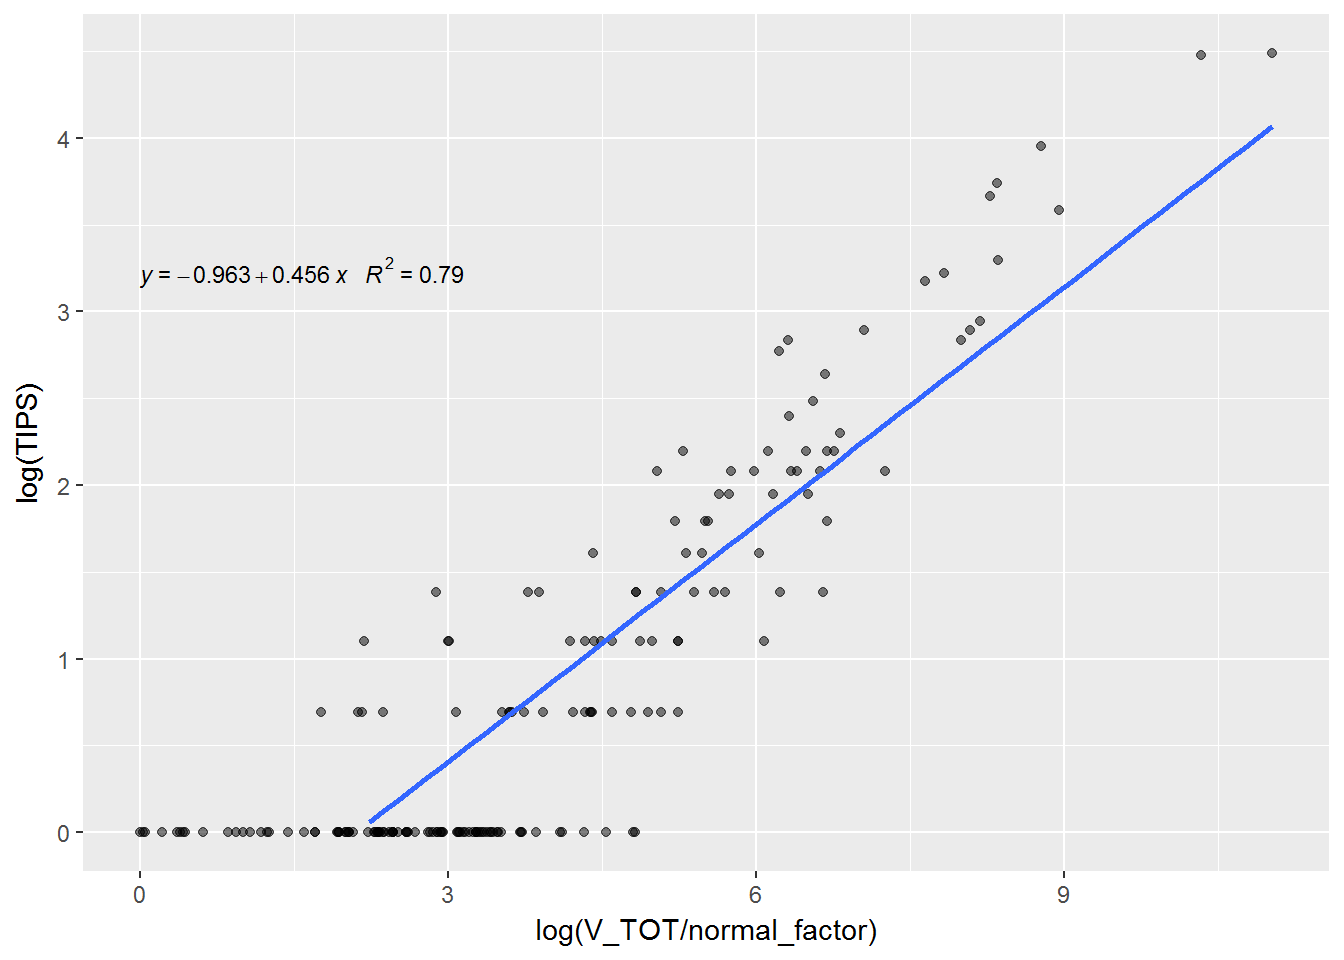
\includegraphics{tip_variability_files/figure-latex/unnamed-chunk-1-1.pdf}
Variance in tip size varys across fifteen orders of magnitude. In a
perfectly symmetrical tree, we would expect the variability in terminal
tips to be 0.

Our primary goal here is to understand the size-dependence of tip
variability so as not to conflate the total size of the trees in the
dataset with the variability in tip sizes. Hopefully this will generate
some insight into volume scaling exponents, to the extent that variation
in volume scaling exponents is influenced by terminal tip variability.
Accordingly, tip variability exhibits scaling with the total size of
trees:

\includegraphics{tip_variability_files/figure-latex/unnamed-chunk-2-1.pdf}

An important pattern emerges: the variance in terminal tip sizes
increases with the size of subtrees as more and more outliers are
included in the tree's distribution of tips. This scaling pattern ends
up being related to our phenomenological volume scaling exponents:

\includegraphics{tip_variability_files/figure-latex/unnamed-chunk-3-1.pdf}

As well as simply the variability in the tips themselves:

\includegraphics{tip_variability_files/figure-latex/unnamed-chunk-4-1.pdf}

What are the quantitative effects of variability in tip volume on volume
scaling exponents? How can we compartmentalize the effects of tree size
on total variability?

\end{document}
